\documentclass[tikz,border=10pt]{standalone}
\usepackage{amsmath,amssymb}
\usepackage{tikz}
\usetikzlibrary{arrows,automata,backgrounds,calendar,chains,decorations,decorations.pathreplacing,decorations.text,fit,matrix,mindmap,patterns,petri,plotmarks,positioning,shadows,shapes,shapes.callouts,shapes.geometric,shapes.misc,spy,trees,calc,intersections,tikzmark,arrows.meta}
\usepackage{xcolor}
\usepackage{pgfplots}
\pgfplotsset{compat=1.16}

% Common math macros from the book
\def\x{\mathbf{x}}
\def\y{\mathbf{y}}
\def\z{\mathbf{z}}
\def\A{\mathbf{A}}
\def\b{\mathbf{b}}
\def\c{\mathbf{c}}
\def\w{\mathbf{w}}
\def\v{\mathbf{v}}
\def\u{\mathbf{u}}
\def\e{\mathbf{e}}
\def\zero{\mathbf{0}}
\def\R{\mathbb{R}}
\def\N{\mathbb{N}}
\def\Z{\mathbb{Z}}
\def\Q{\mathbb{Q}}
\def\st{\text{s.t.}}
\def\vect#1{\mathbf{#1}}
\def\xLP{x^{\mathrm{LP}}}
\def\zLP{z^{\mathrm{LP}}}
\def\xIP{x^{\mathrm{IP}}}

% Common node styles from the book
\tikzset{
    main/.style={circle, draw, fill=gray!20, minimum size=1cm, font=\normalsize},
    dot/.style={circle,fill=blue,minimum size=3pt,inner sep=0pt, outer sep=-1pt},
    vertex/.style={circle,fill=black!25,minimum size=20pt,inner sep=0pt},
    edge/.style={draw,-,thick},
    directed edge/.style={draw,->,>=latex,thick},
}

% Additional macros for 3D/coordinate systems
\newcommand{\xhat}{\hat{\x}}
\newcommand{\yhat}{\hat{\y}}
\newcommand{\zhat}{\hat{\z}}
\newcommand{\ihat}{\hat{\imath}}
\newcommand{\jhat}{\hat{\jmath}}
\newcommand{\khat}{\hat{k}}

\begin{document}
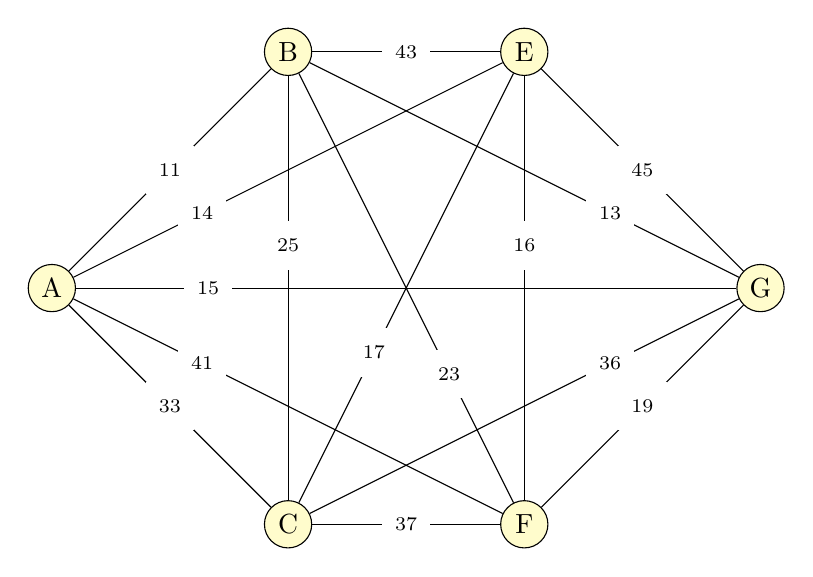
\begin{tikzpicture}[
  every node/.style={circle, draw, fill=yellow!20, minimum size=6mm, inner sep=1pt},
  edge label/.style={font=\scriptsize, rectangle, draw = white, fill=white, inner sep=2pt}
]

% Nodes
\node (A) at (0,0) {A};
\node (B) at (3,3) {B};
\node (C) at (3,-3) {C};
\node (E) at (6,3) {E};
\node (F) at (6,-3) {F};
\node (G) at (9,0) {G};

% Edges with separate edge label style
\draw (A) -- (B) node[midway, edge label] {11};
\draw (A) -- (C) node[midway, edge label] {33};
\draw (A) -- (E) node[pos=0.3, edge label] {14};
\draw (A) -- (F) node[pos=0.3, edge label] {41};
\draw (A) -- (G) node[pos=0.2, edge label] {15};

\draw (B) -- (C) node[pos=0.4, edge label] {25};
\draw (B) -- (E) node[midway, edge label] {43};
\draw (B) -- (F) node[pos=0.7, edge label] {23};
\draw (B) -- (G) node[pos=0.7, edge label] {13};

\draw (C) -- (E) node[pos=0.35, edge label] {17};
\draw (C) -- (F) node[midway, edge label] {37};
\draw (C) -- (G) node[pos=0.7, edge label] {36};

\draw (E) -- (F) node[pos=0.4, edge label] {16};
\draw (E) -- (G) node[midway, edge label] {45};
\draw (F) -- (G) node[midway, edge label] {19};

\end{tikzpicture}
\end{document}
